\documentclass[11pt, a4paper]{article}

\usepackage{amsmath}
\usepackage{amsfonts}
\usepackage{graphicx}
\usepackage[export]{adjustbox}
\usepackage{hyperref}
\usepackage{fullpage}
\usepackage{caption}
\usepackage{listings}
\usepackage[dvipsnames]{xcolor}
\usepackage{gensymb}
\usepackage{wrapfig}
\hypersetup{
    bookmarks=true,         % show bookmarks bar?
    unicode=false,          % non-Latin characters in Acrobat’s bookmarks
    pdftoolbar=true,        % show Acrobat’s toolbar?
    pdfmenubar=true,        % show Acrobat’s menu?
    pdffitwindow=false,     % window fit to page when opened
    pdfstartview={FitH},    % fits the width of the page to the window
    pdftitle={My title},    % title
    pdfauthor={Author},     % author
    pdfsubject={Subject},   % subject of the document
    pdfcreator={Creator},   % creator of the document
    pdfproducer={Producer}, % producer of the document
    pdfkeywords={keyword1, key2, key3}, % list of keywords
    pdfnewwindow=true,      % links in new PDF window
    colorlinks=true,       % false: boxed links; true: colored links
    linkcolor=Blue,          % color of internal links (change box color with linkbordercolor)
    citecolor=green,        % color of links to bibliography
    filecolor=magenta,      % color of file links
    urlcolor=red           % color of external links
}

\title{MAAS - Street Network Visualization \\Commitment Issues}
\author{Sushant Vijay Chavan\\Ahmed Faisal Abdelrahman\\Abanoub Abdelmalak}
\date{\today}

\begin{document}
\maketitle
\newpage
\tableofcontents{}
\newpage

\section{Introduction}
\paragraph{}


\newpage
\subsection{Graph Visualization Agent (Developer: All)}\label{GraphVisualizationAgent}
\paragraph{}
The graph visualization agent facilitates observing the delivery process of the orders in a graphical way. This agent is capable of displaying the entire street network (consisting of its nodes and edges) and all the trucks present at any given time as shown in figure \ref{VisualizationScreenshot}. JavaFX was used to generate the nice display and we used and modified the implementation of \href{https://stackoverflow.com/a/30696075}{Roland} to generate the graph representation.

\begin{figure}[h!]
	\centering
	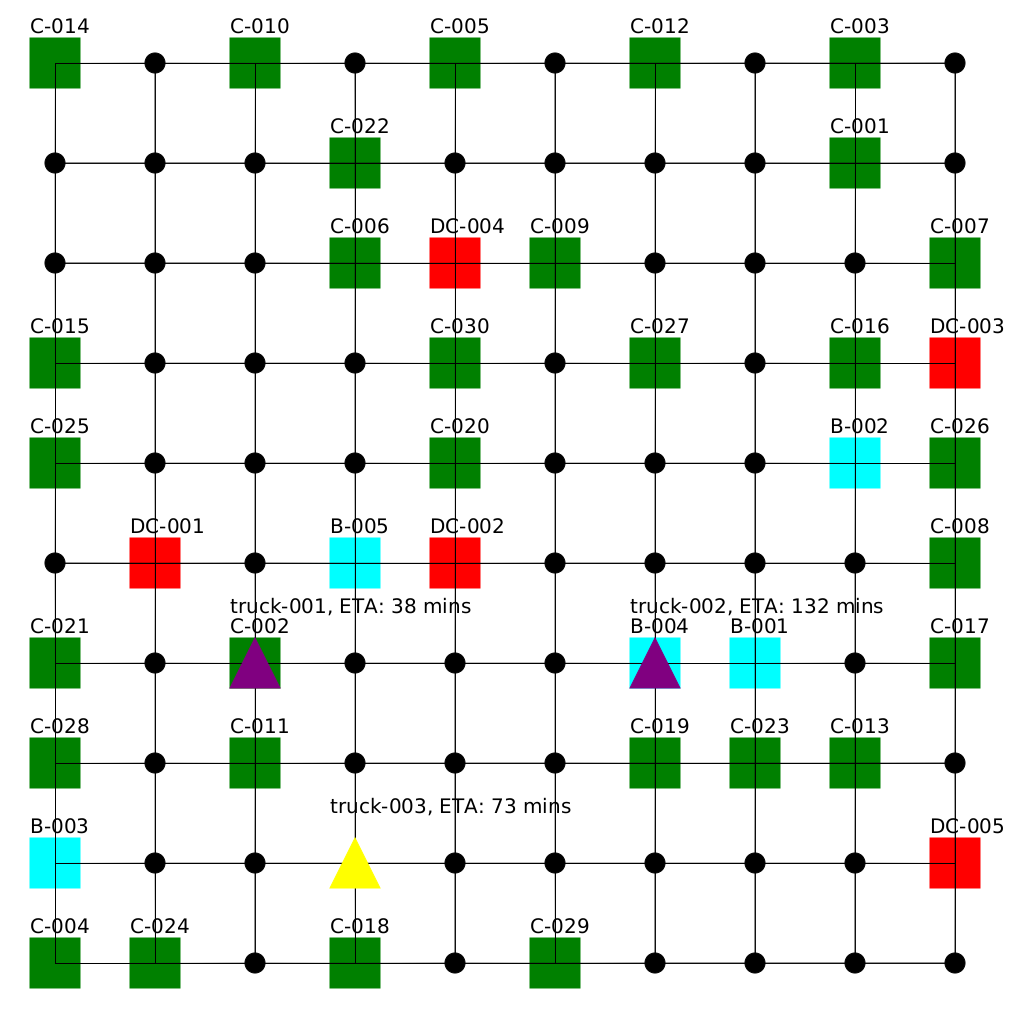
\includegraphics[width=\textwidth]{Visualization.png}
	\caption{Screenshot of Delivery Stage Visualization}
	\label{VisualizationScreenshot}
\end{figure}


\end{document}\grid
